\chapter{Abituraufgabe 2023-1}\label{aufg:2023-1}

\section{Fachliche Grundlagen}

\subsection{Entfernungsmessungen}
\label{chap:Entfernung}
In der Astronomie gibt es verschiedene Möglichkeiten zur Bestimmung der Entfernung von Objekten im Weltall. Eine Möglichkeit ist die Parallaxemethode. Diese wird zum Beispiel für die Entfernungsbestimmung naher Sterne verwendet. Der Grundgedanke ist, dass diese Sterne sich aus Sicht der Erde vor einem Hintergrund aus Fixsternen befindet. Im Laufe eines Jahres betrachtet man den Stern aus unterschiedlichen Winkeln, da die Erde auf ihrem Orbit eine Strecke von circa \SI{2}{\astronomicalunit} zurücklegt. Das äußert sich darin, dass der Stern vor dem Hintergrund verschoben wird.
Der Winkel $\varphi$, um den der Stern verschoben zu sein scheint, wird Parallaxewinkel genannt. Das Prinzip ist in \cref{fig:Parallaxe} veranschaulicht. 
\begin{figure}
	\centering
	\begin{tikzpicture}
		\coordinate(orig) at (0,0);
		\coordinate (one) at (0,-1.5);
		\coordinate (two) at (0,1.5);
		\coordinate (star) at (5,0);
		\coordinate (fix1) at (10,3);
		\coordinate (fix2) at (10,2);
		\coordinate (fix3) at (10,0);
		\coordinate (fix4) at (10,-1);
		\coordinate (fix5) at (10,-3);
		
		
		\draw[fill=yellow](orig) circle (0.25) node[label={[label distance=0.15cm]270:Sonne}] {};
		\draw[fill=yellow](star) circle (0.25) node[label={[label distance=0.15cm]270:Stern}] {};
		\draw[fill=yellow](fix1) circle (0.25);
		\draw[fill=yellow](fix2) circle (0.25);
		\draw[fill=yellow](fix3) circle (0.25);
		\draw[fill=yellow](fix4) circle (0.25);
		\draw[fill=yellow](fix5) circle (0.25) node[label={[label distance=0.15cm]270:Fixsterne}] {};
		\draw (orig) circle (1.5);
		
		\draw[dashed] (one) -- ++(10,3);
		\draw[dashed] (two) -- ++(10,-3) node (end){};
		\draw[<->] (orig) -- (2.5,0) node[below] {$d$} -- (star);
		\draw[<->] (orig) -- (0,0.75) node[right] {\SI{1}{\astronomicalunit}}-- (two) ;
		\draw[dashed] (star)--(fix3);
		\draw pic [draw, "$\varphi$", angle radius = 2cm]{angle = two--star--orig};
		\draw pic [draw, "$\varphi$", angle radius = 2cm]{angle = end--star--fix3};
		\draw[text=black,draw=black,fill=white] (one) circle (0.25) node{1};
		\draw[text=black,draw=black,fill=white] (two) circle (0.25) node{2};
	\end{tikzpicture}
	\caption{Veranschaulichung der Parallaxemethode. Der Parallaxewinkel $\varphi$ eines Sternes wird durch Messungen im Abstand eines halben Jahres gemessen. Daraus kann der Abstand $d$ berechnet werden.}
	\label{fig:Parallaxe}
\end{figure}
Misst man mit einem Teleskop den Winkel $\varphi$, so kann man aus dem Abstand von Sonne und Erde den Abstand $d$ des Sterns berechnen. Es gilt dann mit der Kleinwinkelnäherung
\begin{align*}
	\varphi&\approx \tan(\varphi)=\frac{\SI{1}{\astronomicalunit}}{d}\\
	d&= \frac{\SI{1}{\astronomicalunit}}{\varphi}
\end{align*}
Auf diese Weise kann man eine neue Längeneinheit definieren, das Parsec (\unit{\parsec}). Es handelt sich um den Abstand, den ein Stern hätte, wenn er einen Parallaxewinkel von einer Bogensekunde ($\SI{1}{\arcsecond}=\SI{1}{\arcsec}$) hätte. Der Name besteht daher aus \enquote{Parallaxe} und \enquote{arcsec}. Rechnet man die Parallaxe in Bogensekunden um, so nennt man sie $p$ und der Abstand $d_{\text{\unit{\parsec}}}$ in \unit{\parsec} ist gegeben durch:
\begin{align*}
	d_{\text{\unit{\parsec}}}&=\frac{\SI{1}{\arcsecond}}{p}
\end{align*}

Eine andere Möglichkeit zur Berechnung der Entfernung ist das Entfernungsmodul. Mit dieser Methode können Entfernungen von Objekten bestimmt werden, die zu geringe Parallaxen haben, um die mit den verfügbaren Teleskopen aufzulösen. Dabei verwendet man die scheinbare Helligkeit $m$ und absolute Helligkeit $M$ von Sternen. Die scheinbare Helligkeit des Sternes ist von seinem Abstand abhängig (vgl. \cref{chap:Intensität}). Die absolute Helligkeit ist definiert als scheinbare Helligkeit in einem Abstand von $\SI{10}{\parsec}$. Die scheinbare Helligkeit kann von der Erde aus gemessen werden. Die absolute Helligkeit muss man auf andere Weisen bestimmen, zum Beispiel durch Pulsare, Standardkerzen und charakteristische Spektren des Sternenlichtes. Hat man beide dieser Werte experimentell bestimmt, so kann man die Formel des Entfernungsmoduls verwenden~\cite[S.17]{Cornelsen2013} und nach dem Abstand $d$ auflösen:
\begin{align*}
	m-M&=5\cdot \lg(\frac{d}{\SI{10}{\parsec}})\\
	\frac{m-M}{5}&=\lg(\frac{d}{\SI{10}{\parsec}})\\
	10^{\frac{m-M}{5}}&=\frac{d}{\SI{10}{\parsec}}\\
	\frac{d}{\unit{\parsec}}&=10\cdot10^{\frac{m-M}{5}}\\
	d_{\text{\unit{\parsec}}}&=10^{\frac{m-M}{5}+1}.
\end{align*}

\subsection{Sternenlicht}
\label{chap:Intensität}
Für die Entfernungsbestimmung mit dem Entfernungsmodul ist eine Kenntnis über die Helligkeit eines Sternes notwendig. Diese hängt mit der Lichtstrahlung des Sternes zusammen. Deshalb sollen hier die wesentlichen Begriffe im Zusammenhang mit dem Sternenlicht voneinander abgegrenzt werden.
Die Leuchtkraft $L$ bezeichnet die Strahlungsleistung des Sternes und hat damit die Einheit Watt (\unit{\watt}). Es handelt sich um die gesamte Energie, die der Stern pro Sekunde in den gesamten Raum abstrahlt. Diese Größe hängt daher nicht von der Entfernung oder der Betrachtung ab. Sie ist allein durch die Energieproduktion durch Kernfusion im Inneren des Sternes gegeben. Die Leuchtkraft setzt sich aus allen Wellenlängen zusammen, ist also das Ergebnis eines Integrals über die spektrale Leistungsdichte. Diese bezeichnet die Leistung pro Wellenlänge und ist durch das Planck'sche Strahlungsgesetz gegeben. Sie ist daher von der Temperatur des Sternes abhängig. Die Temperaturabhängigkeit der Strahlungsdichte ist in \cref{fig:Planck} veranschaulicht.
\begin{figure}
	\centering
	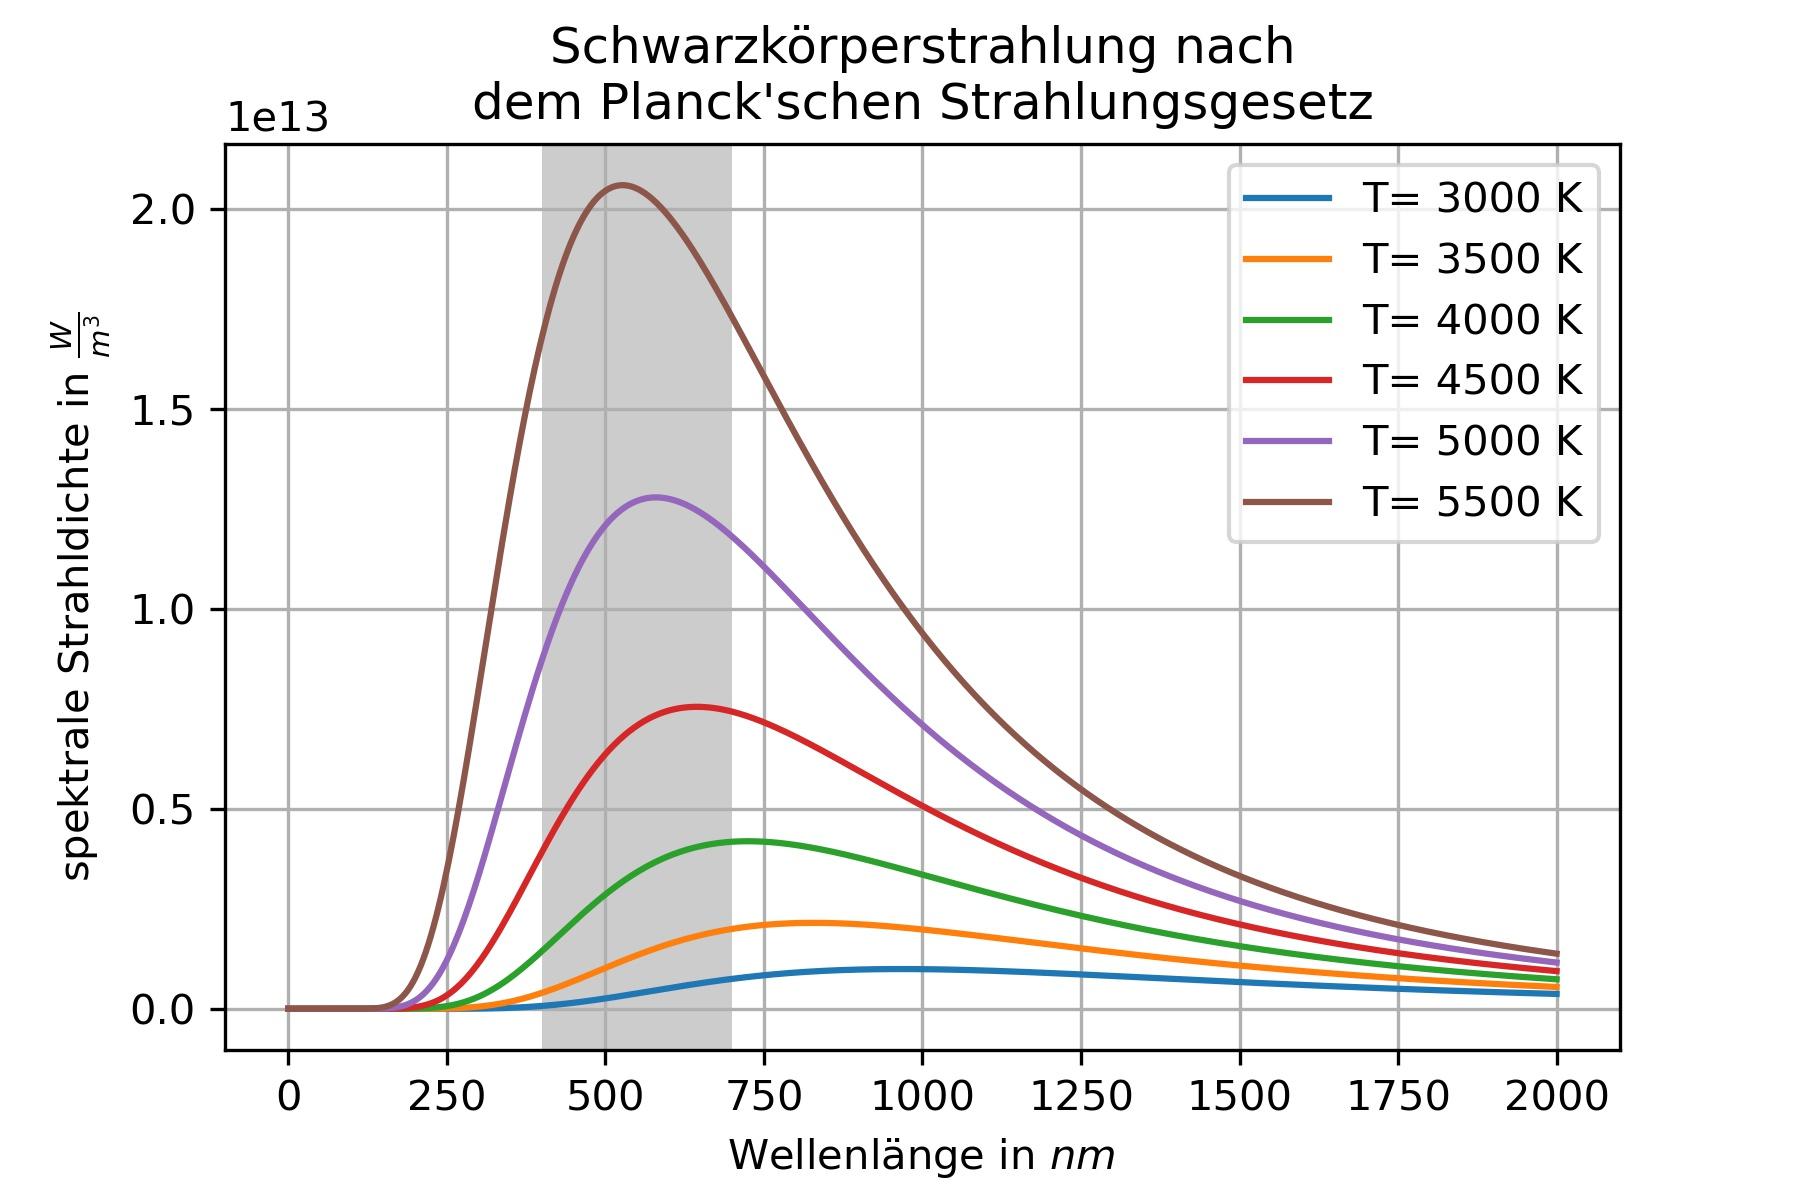
\includegraphics[width= 0.6\textwidth]{Bilder/Planck.jpg}
	\caption{Spektrale Strahlungsdichte eines schwarzen Körpers nach dem Planck'schen Strahlungsgesetz. Die Linien zeigen die Spektren für Temperaturen, die für die Sterne in dieser Aufgabe passen. Das grau hinterlegte Intervall ist der Wellenlängenbereich von sichtbarem Licht. Man sieht, dass Sterne unter \SI{3e3}{\kelvin} hauptsächlich im infraroten Spektralbereich strahlen. Die Strahlungsdichte hat die Einheit \unit{\watt \per \meter \cubed}, weil noch über die Fläche und die Wellenlänge integriert werden muss. Dann erhält man die Leuchtkraft mit der Einheit \unit{\watt}.}
	\label{fig:Planck}
\end{figure}
Insgesamt ergibt sich für die Leuchtkraft eines Sternes jedoch eine sehr einfache Formel, die nur noch von der Temperatur $T$ und der Oberfläche des Sternes $A=4\cdot\pi\cdot r^2$ abhängt~\cite[S.16]{Cornelsen2013}:
\begin{align*}
	L&=A\cdot\sigma\cdot T^4
\end{align*}
mit der Stefan-Boltzmann-Konstante $\sigma$.

Ist man daran interessiert, welche Leistung auf einem Planeten in einiger Entfernung ankommt, dann muss man auch den Abstand des Planeten berücksichtigen. Dann ist die Bestrahlungsstärke $E$ die relevante Größe. Sie ist eine Leistung pro Fläche, hat also die Einheit \unit{\watt \per \meter \squared}. Da die Sterne in alle Richtungen etwa gleich abstrahlen, verteilt sich in einem gegebenen Abstand $d$ die gesamte Leuchtkraft auf eine Kugeloberfläche mit Radius $d$. Damit wird für zunehmenden Abstand die Bestrahlungsstärke quadratisch abfallen, denn es gilt:
\begin{align*}
	E= \frac{L}{4\cdot\pi\cdot d^2}.
\end{align*}
Die Leistung die ein Planet dann absorbieren kann ist das Produkt von Bestrahlungsstärke $E$ und seiner Fläche $A$, die der Stern von ihm sieht. Das ist eine Kreisscheibe mit dem Radius $R$ des Planeten. Damit gilt für die absorbierte Leistung unter Vernachlässigung von Reflexion:
\begin{align*}
	P_{\text{Planet}}=E\cdot \pi \cdot R^2= \frac{L}{4}\cdot \qty(\frac{R}{d})^2.
\end{align*}


\subsection{Zweikörperproblem}

Die Beschreibung von Planetenbahnen hat eine lange Geschichte. Mit Keplers Gesetzen wurde empirisch bestimmt, dass sich die Planeten des Sonnensystems auf Ellipsen um die Sonne bewegen. Eine theoretische Beschreibung, die mit diesen Bahnen übereinstimmte lieferte erst die Newton'sche Kräftemechanik. Betrachtet man zwei isolierte Körper, auf die nur die Gravitationskraft wirkt, so spricht man von einem Zweikörpersystem und dem Zweikörperproblem. Die Berechnung der Trajektorien ist in guter Übereinstimmung mit den Ellipsenbahnen der meisten Planeten und liefert auch quantitative Beziehungen über die Bewegung der Planeten. Da dieses Problem sehr allgemein formuliert und gerechnet werden kann, gelten die erhaltenen Formeln für alle Zweikörpersysteme auch jenseits des Sonnensystems. Berücksichtigt man die Gravitation eines dritten Körpers, so spricht man vom Dreikörperproblem, welches nur näherungsweise und nicht exakt gelöst werden kann. Im Zweikörperproblem ergeben sich drei mögliche Bahnformen: Ellipsen, Parabeln und Hyperbeln. Liegt eine Ellipse vor, so entfernen sich die zwei Körper nie ins unendliche und man spricht von einem gebundenen System. Parabelbahnen entsprechen dem Grenzzustand ungebundender Bahnen, die ansonsten Hyperbelförmig sind. Die Geschwindigkeit eines Körpers, die notwendig ist um eine ungebundene Bahn zu haben, nennt man Fluchtgeschwindigkeit.

\subsection{Dopplereffekt}

Der Dopplereffekt von Schallwellen ist ein Alltagseffekt, der besonders prägnant auftritt, wenn ein Fahrzeug mit Martinshorn an einem ruhenden Hörer vorbeifährt. Zunächst bewegt sich das Fahrzeug auf den Hörer zu. Dann klingen die beiden Töne des Martinshorns höher, als wenn es den Hörer passiert hat und sich entfernt. Den gleichen Effekt gibt es auch für Licht und man spricht vom optischen Dopplereffekt. Auch dort werden Lichtwellen zu höheren Frequenzen oder \enquote{in's Blaue} verschoben, wenn sich der Emitter auf den Beobachter zu bewegt. Bei einer Geschwindigkeit weg vom Beobachter ist das Licht \enquote{rotverschoben}, also zu niedrigeren Frequenzen. Durch eine genaue Messung von charakteristischen Wellenlängen von Atomen und Molekülen kann damit auf die Bewegung des Emitters also z.B. eines Sterns geschlossen werden.


\section{Musterlösung}

\begin{hinweis}
	In dieser Lösung werden Formeln und physikalische Größen aus einer Formelsammlung~\cite{Cornelsen2013} verwendet, die im achtjährigen Gymnasium zugelassen war. Die Angaben sind beispielhaft zu sehen, da die verwendeten Informationen auch in anderen Formelsammlungen zu finden sind.
\end{hinweis}

\subsection{Proxima Centauri}

\begin{aufgabe}
	\textbf{1. Proxima Centauri}\newline
	Im Sternbild Centaurus wurde 1915 ein lichtschwacher rötlicher Stern entdeckt, der der nächstgelegene Stern zur Sonne ist. Dieser Stern wird daher Proxima Centauri genannt.

	Proxima Centauri hat eine jährliche Parallaxe von \SI{0.768}{\arcsecond}. Im sichtbaren Spektralbereich wird eine scheinbare Helligkeit von \num{11.1} beobachtet.
	\begin{enumerate}
	 	\item Bestimmen Sie die Entfernung von Proxima Centauri zur Erde. Ermitteln Sie seine Leuchtkraft $L_{\text{sichtbar}}$ im sichtbaren Spektralbereich in Vielfachen der Sonnenleuchtkraft.\hfill [Zur Kontrolle: $L_{\text{sichtbar}}=\num{5.3e-5}L_{\odot}$]\newline \hfill S3,S7 / II
	\end{enumerate}
	Bei Proxima Centauri handelt es sich um einen Hauptreihenstern mit der Oberflächentemperatur \SI{3.0e3}{\kelvin}. Sein Durchmesser beträgt \SI{15}{\percent} des Sonnendurchmessers.
	\begin{enumerate}[resume]
	 	\item Berechnen Sie die Gesamtleuchtkraft $L$ von Proxima Centauri in Vielfachen der Sonnenleuchtkraft. Vergleichen Sie dieses Ergebnis mit dem in Teilaufgabe a ermittelten Wert für die Leuchtkraft im sichtbaren Spektralbereich und geben Sie eine Begründung für diese Abweichung an.\hfill [Zur Kontrolle: $L=\num{1.6e-3}L_\odot$]\newline \hfill S1,S7 / II
	\end{enumerate}
\end{aufgabe}


\begin{enumerate}
	\item Wenn die jährliche Parallaxe angegeben ist, kann diese verwendet werden, um direkt den Abstand in Parsec(\unit{\parsec}) anzugeben. Nähere Erklärungen sind in \cref{chap:Entfernung} zu finden. Die notwendige Formel ist auch in der Formelsammlung~\cite[S.17]{Cornelsen2013} zu finden. Mit der Parallaxe $p$ aus der Angabe gilt für den Abstand $d_{PC}$:
	\begin{align*}
		\frac{d_{\text{PC}}}{\SI{1}{\parsec}}&=\frac{\SI{1}{\arcsecond}}{p}\\
		d_{\text{PC}}&=\frac{1}{\num{0.768}}\unit{\parsec}\\
		&=\SI{1.30}{\parsec}
	\end{align*}
	Dabei wurde das Ergebnis auf 3 gültige Ziffern gerundet. Mit den verschiedenen Umrechnungen könnte der Abstand auch in anderen Einheiten angegeben werden. Das ist in dieser Aufgabe nicht explizit verlangt und für die weiteren Teile nicht nötig. 

	Mit dem bekannten Abstand kann nun über Zwischenschritte die Leuchtkraft $L_{\text{sichtbar}}$ im sichtbaren Licht berechnet werden. Die scheinbare Helligkeit $m$ ist aus historischen Gründen auf das sichtbare Licht bezogen und kann dazu verwendet werden. Mit der scheinbaren Helligkeit und dem Abstand des Sternes kann das Entfernungsmodul~\cite[S.17]{Cornelsen2013} verwendet werden, um die absolute Helligkeit $M$ zu berechnen. Die absoluten Helligkeiten zweier Sterne können verglichen werden, um die Leuchtstärken zu vergleichen, wie es hier das Ziel ist. Es gilt:
	\begin{align*}
		m-M&=5\cdot\lg(\frac{d_{\text{PC}}}{\SI{10}{\parsec}})\\
		M&=m-5\lg(\num{0.130})\\
		&=\num{11.1}-(-\num{4.43})\\
		&=\num{15.5}
	\end{align*}
	Dabei wurde das Ergebnis auf 3 gültige Ziffern gerundet. Die absolute Helligkeit kann nun mit der absoluten Helligkeit $M_\odot$ der Sonne verglichen werden. Damit erhält man das Verhältnis der Leuchtstärken. Mit dem Wert $M_\odot = \num{4.83}$~\cite[S.46]{Cornelsen2013} und der Formel aus~\cite[S.17]{Cornelsen2013} erhält man:
	\begin{align*}
		M-M_\odot&=-\num{2.5}\lg(\frac{L_{\text{sichtbar}}}{L_\odot})\\
		\lg(\frac{L_{\text{sichtbar}}}{L_\odot})&=-\frac{2}{5}(M-M_\odot)\\
		\frac{L_{\text{sichtbar}}}{L_\odot}&=10^{-\frac{2}{5}(M-M_\odot)}\\
		\frac{L_{\text{sichtbar}}}{L_\odot}&=10^{-\frac{2}{5}(\num{15.5}-\num{4.83})}=\num{5.40e-5}\\
		L_{\text{sichtbar}}&=\num{5.40e-5}L_\odot
	\end{align*}
	Das Ergebnis stimmt in etwa mit dem Kontrollergebnis ein. Zudem kann man noch eine kurze Plausibilitätsüberlegung anstellen: der Stern hat eine Parallaxe von etwas unter $\SI{1}{\arcsecond}$, sollte also etwas weiter als $\SI{1}{\parsec}$ entfernt sein. Seine scheinbare Helligkeit ist aufgrund der großen Magnitude eher gering, und sie wird noch geringer, wenn man sich bis auf $\SI{10}{\parsec}$ entfernt. Insgesamt kann man daher mit einer Leuchtkraft rechnen, die deutlich unter der der Sonne liegt.



	\item In der letzten Teilaufgabe wurde nur die Strahlungleistung im sichtbaren Bereich berücksichtig. Das liegt daran, dass die scheinbare Helligkeit historisch gesehen auf Beobachtungen im sichtbaren Spektrum zurückgeht. Das Spektrum von Sternen ist jedoch ein Schwarzkörperspektrum und damit wird von Sternen auch Licht abgestrahlt, was mit dem Auge nicht sichtbar ist. Die gesamte Leuchtkraft über alle Spektralbereiche ist daher unter Umständen höher. Die gesamte Strahlungsleistung ergibt sich aus dem Stefan-Boltzmann-Gesetz~\cite[S.16]{Cornelsen2013}
	\begin{align*}
		L&=A\cdot\sigma\cdot T^4
	\end{align*}
	mit der Fläche $A$, der Temperatur $T$ in Kelvin und der Stefan-Boltzmann-Konstante $\sigma$. Da die Oberflächentemperaturen und Radien von Proxima Centauri und der Sonne bekannt sind, kann man ihre Leuchtkräfte ins Verhältnis setzen. Dabei verwendet man $A=4\cdot\pi\cdot r^2$~\cite[S.69]{Cornelsen2013}:
	\begin{align*}
		\frac{L}{L_\odot}&=\frac{A\cdot \sigma \cdot T^4}{A_\odot \cdot \sigma \cdot T_\odot^4}\\
		&=\frac{4\pi r^2\cdot \sigma \cdot T^4}{4\pi r_\odot^2\cdot \sigma \cdot T_\odot^4}\\
		&=\qty(\frac{r}{r_\odot})^2\cdot \qty(\frac{T}{T_\odot})\\
		\intertext{Mit $T_\odot$ = \SI{5.8e3}{\kelvin}~\cite[S.47]{Cornelsen2013} folgt dann:}\\
		\frac{L}{L_\odot}&=(\num{0.15})^2\cdot\qty(\frac{\num{3}}{\num{5.8}})^4=\num{1.61e-3}\\
		L&=\num{1.6e-3}L_\odot
	\end{align*}
	Dabei wurde das Endergebnis auf 2 gültige Ziffern gerundet. Wie eingangs beschrieben, fällt die gesamte Strahlungleistung von Proxima Centauri deutlich höher aus als die visuelle. Das liegt daran, dass der Stern hauptsächlich im Infraroten Spektralbereich strahlt. Das kann man mit dem Wien'schen Verschiebungsgesetz~\cite[S.16]{Cornelsen2013} und dem Wert für die Wien'sche Verschiebungskonstante $b$~\cite[S.42]{Cornelsen2013} sehen:
	\begin{align*}
		\lambda_{\text{max}}\cdot T&=b\\
		\lambda_{\text{max}}&=\frac{b}{T}\\
		&=\frac{\SI{2.8978e-3}{\meter \kelvin}}{\SI{3.0e3}{\kelvin}}\\
		&=\SI{966}{\nano \meter}
	\end{align*}
	Die Wellenlänge mit der maximalen Strahlungsleistung $\lambda_{\text{max}}$ liegt also deutlich unterhalb der Grenze des sichtbaren Lichtes bei circa \SI{700}{\nano\meter} und damit im Infraroten.
\end{enumerate}

\subsection{Proxima Centauri und das Doppelsternsystem Alpha Centauri}

\begin{aufgabe}[sidebyside, sidebyside align = top,righthand width=3cm]
	\textbf{2. Proxima Centauri und das Doppelsternsystem Alpha Centauri}\newline
	
	Proxima Centauri scheint sich um das Doppelsternsystem Alpha Centauri zu bewegen, welches näherungsweise als ein Zentralgestirn mit \num{2.16} Sonnenmassen angenommen werden kann. Die Masse von Proxima Centauri ist gegenüber der Masse von Alpha Centauri vernachlässigbar klein.

	Für Proxima Centauri wurden in den letzten Jahren verschiedene Bahnformen diskutiert, von denen zwei in \cref{fig:Proxima-Orbit} aus Sicht der Erde mit der momentanen Position von Proxima Centauri dargestellt sind. Die große Halbachse der elliptischen Bahn 1 beträgt \SI{9e3}{\astronomicalunit}.
	

	\begin{enumerate}
	 	\item Berechnen Sie die Umlaufzeit von Proxima Centauri auf Bahn 1.\newline
		 \hfill [Zur Kontrolle: \SI{6e5}{\year}]\newline \hfill S7 / I
		\item Begründen Sie, dass trotz 100-jähriger Beobachtung nicht geklärt werden konnte, ob sich Proxima Centauri auf Bahn 1 oder auf Bahn 2 bewegt. Schätzen Sie mithilfe von \cref{fig:Proxima-Orbit} grob ab, in wie vielen Jahren eine Momentaufnahme des Centauri-Systems genügen wird, um eine der Bahnen auszuschließen. Gehen Sie dabei von einem konstanten Betrag der Bahngeschwindigkeit aus.\newline \hfill S7,K3 / I
	\end{enumerate}
	Neueste Beobachtungsdaten von Alpha Centauri und Proxima Centauri ermöglichen sehr präzise Geschwindigkeitsbestimmungen und stützen die Annahme, dass es sich bei Alpha Centauri und Proxima Centauri um ein gravitativ gebundenes System handelt. Proxima Centauri ist heute \SI{13e3}{\astronomicalunit} von Alpha Centauri entfernt.
	\begin{enumerate}[resume]
	 	\item Bestimmen Sie für einen Körper an der heutigen Position von Proxima Centauri die Geschwindigkeit, die er zum Verlassen des gravitativen Einflussbereichs von Alpha Centauri benötigt, also die 2. kosmische Geschwindigkeit. Beschreiben Sie unter Verwendung Ihres Ergebnisses ein Kriterium, das die Wissenschaftlerinnen und Wissenschaftler in der Annahme eines gebundenen Systems bestärkt haben könnte.\newline \hfill S1,S7 / I
	\end{enumerate}
	\tcblower
		\centering
		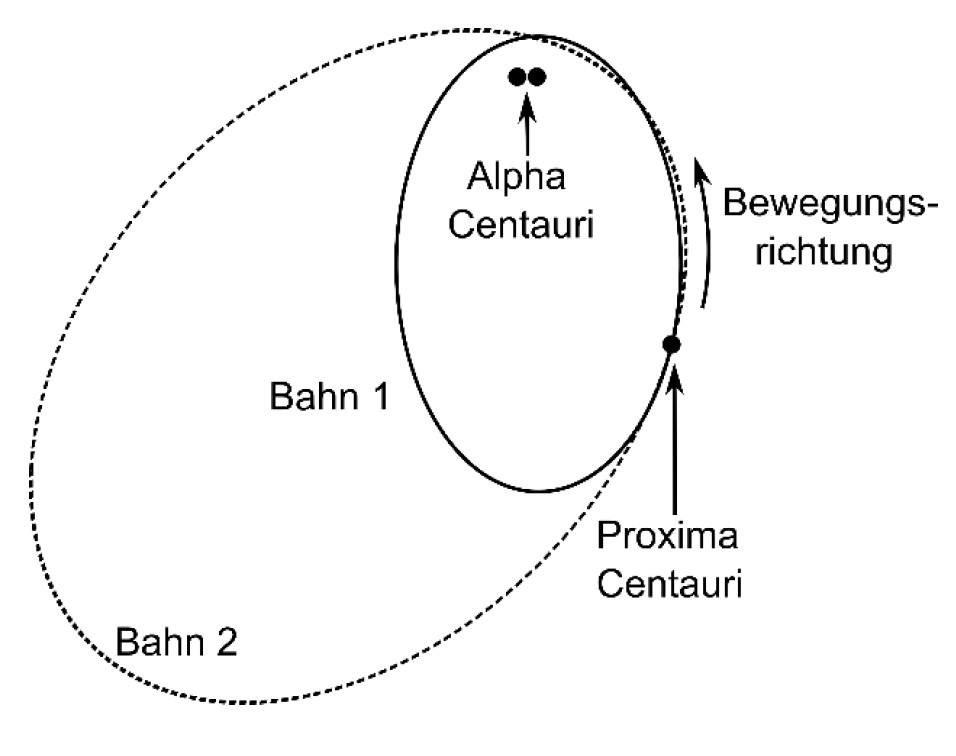
\includegraphics[width=0.3\textwidth]{Bilder/Proxima_orbits.jpg}{}
		\captionof{figure}{}\label{fig:Proxima-Orbit}
\end{aufgabe}

\begin{enumerate}
	\item Die Umlaufzeit von Planeten kann durch Lösung des Zweikörperproblemes berechnet werden. Ist die Masse eines der beiden Körper viel größer, als die des anderen, kann man die Formeln deutlich vereinfachen. Der Zusammenhang zwischen Umlaufdauer $T$ und großer Ellipsenhalbachse $a$ ist dann gegeben durch~\cite[S.15]{Cornelsen2013}:
	\begin{align*}
		\frac{T^2}{a^3}&=\frac{4\pi^2}{GM_\alpha}
	\end{align*}
	mit der Masse $M_\alpha$ des Sterns Alpha Centauri. Diese Formel kann umgeformt werden, um die Umlaufdauer zu berechnen. Dabei werden die Werte für die Gravitationskonstante $G$~\cite[S.42]{Cornelsen2013}, die Sonnenmasse~\cite[S.47]{Cornelsen2013} und die Definition der Astronomischen Einheit \unit{\astronomicalunit}~\cite[S.45]{Cornelsen2013} benutzt:
	\begin{align*}
		\frac{T^2}{a^3}&=\frac{4\pi^2}{GM_\alpha}\\
		T^2&=\frac{4\pi^2}{GM_\alpha}\cdot a^3\\
		T&=\sqrt{\frac{4\pi^2}{GM_\alpha}\cdot a^3}\\
		&=\sqrt{\frac{4\pi^2}{G\cdot\num{2.16}M_\odot}\cdot (\SI{9e3}{\astronomicalunit})^3}\\
		&=\sqrt{\frac{4\pi^2}{\SI{6.67e-11}{\meter\cubed\per\kg\per\second\squared}\cdot\num{2.16}\cdot\SI{1.989e30}{\kg}}\cdot (\num{9e3}\cdot\SI{1.496e11}{\meter})^3}\\
		&=\SI{1.833e13}{\second}=\frac{\num{1.833e13}}{\num{31556952}}\unit{\year}\\
		&\approx\SI{6e5}{\year}
	\end{align*}
	Damit wurde verwendet, dass ein Jahr \SI{3155693}{\second} hat ~\cite[S.45]{Cornelsen2013}.
	\item Um nachvollziehen zu können, dass die Entscheidung zwischen den beiden Bahnen noch nicht getroffen werden konnte, berechnen wir die Distanz, die Proxima Centauri in 100 Jahren zurück legt, wenn es sich gleichförmig bewegen würde. Nimmt man an, dass die Zeichnung maßstabsgetreu ist, so kann man den Abstand $r_{\text{PC}}$ grob abschätzen. Hier kommt es nicht auf den genauen Wert an, deshalb schätzen wir $r_{\text{PC}}\approx a$. Für die Bahngeschwindigkeit $v$ eines Himmelskörpers auf einer Keplerellipse gilt~\cite[S.14]{Cornelsen2013}:
	\begin{align*}
		v&=\sqrt{GM\qty(\frac{2}{r}-\frac{1}{a})}\\
		\intertext{und damit im vorliegenden Fall}
		v&=\sqrt{GM_\alpha\qty(\frac{2}{a}-\frac{1}{a})}\\
		&=\sqrt{GM_\alpha\frac{1}{a}}\\
		&=\sqrt{\SI{6.67e-11}{\meter\cubed\per\kg\per\second\squared}\cdot\num{2.16}\cdot\SI{1.989e30}{\kg}\frac{1}{\num{9e3}\cdot \SI{1.4989e11}{\meter}}}\\
		&=\SI{461.3}{\meter\per\second}\\
		v&\approx\SI{0.5}{\kilo\meter\per\second}
	\end{align*}
	\begin{hinweis}
		An dieser Stelle kann man beispielhaft eine Überschlagsrechnung der Größenordnungen durchführen. Das ist eine gute Möglichkeit, um Ergebnisse aus Taschenrechnereingaben zu kontrollieren. In der wissenschaftlichen Notation werden Größen in der Form $\num{1000}=\num{e3}$ angegeben. Bei Multiplikation solcher Zahlen addieren sich die Exponenten, also $\num{e3}\cdot\num{e5}=\num{e8}$ oder $\num{e4}\cdot\num{e-2}=\num{e2}$. Beim Wurzelziehen wird der Exponent halbiert und beim quadrieren verdoppelt. Für die vorliegende Rechnung ergibt sich unter Berücksichtigung der Zehnerpotenzen ein Exponent von 
		\begin{align*}
			\frac{-11+30-4-11}{2}=2
		\end{align*}
		Man kann also damit rechnen, dass in SI-Einheiten eine Zahl der Größenordnung $\num{e2}=\num{100}$ herauskommt, und das Ergebnis stimmt damit gut überein.
	\end{hinweis}
	Da wir eine gleichförmige Bewegung annehmen gilt für die zurückgelegte Strecke~\cite[S.10]{Cornelsen2013}:
	\begin{align*}
		\Delta s &= v \cdot \Delta t\\
		&=\SI{0.5}{\kilo\meter\per\second}\cdot \num{100} \cdot \SI{31556952}{\second}\\
		&\approx\SI{1.6e9}{\kilo\meter}=\frac{\num{1.6e9}}{\num{1.496e8}}\unit{\astronomicalunit}\\
		&\approx\SI{11}{\astronomicalunit}
	\end{align*}
	Dieser Wert ist nur ein Bruchteil der Hauptachse, also hat der Stern in den letzten 100 Jahren nur einen kleinen Winkel seiner Ellipse überstrichen. Daher ist es nicht verwunderlich, dass die Entscheidung über die tatsächliche Bahn noch aussteht, weil die beiden Kandidaten sich in diesem Bereich kaum unterscheiden. Betrachtet man die Skizze, so muss ein deutlich größerer Winkel überstrichen werden. Geht man von einer genauen Ortsbestimmung aus, so kann man bei der Teilung der Bahnen etwa \ang{20} von der jetztigen Position von einer Entscheidung ausgehen. Bei ungenauer Ortsbestimmung unter Umständen sogar erst bei Winkeln um \ang{70}.
	Geht man davon aus, dass die Entscheidung bei einer Bewegung um weitere \ang{20} getroffen werden kann, so kann man grob von gleichbleibendem Tempo ausgehen. Dann ist die Dauer $\frac{20}{360}$ der gesamten Umlaufzeit und damit
	\begin{align*}
		\Delta t &=\frac{20}{360}\cdot T \approx \SI{3.3e5}{\year}.
	\end{align*}

	\item Die 2. kosmische Geschwindigkeit wird auch als Fluchtgeschwindigkeit bezeichnet. Für einen Körper, der unter dem gravitativen Einfluss eines anderen Körpers steht, ist diese Geschwindigkeit nötig, um sich für immer von dem Körper zu entfernen. Die Gravitation reicht dann nicht mehr aus, um die beiden Körper in einem Orbit zu halten. Die Fluchtgeschwindigkeit bezieht sich üblicherweise auf die Oberfläche eines kugelförmigen Körpers. Man kann sich eine Kugel denkten, deren Radius genau der Abstand $r_{\text{PC}}$ von Proxima Centauri und Alpha Centauri ist. Diese Kugel soll Alpha Centauri im Zentrum haben und die gleiche Masse $M_\alpha$ haben. Die Fluchtgeschwindigkeit von Proxima Centauri bezüglich Alpha Centauri kann dann mit dieser fiktiven Kugel abgeschätzt werden und alle Bedingungen für die Formel~\cite[S.15]{Cornelsen2013} sind erfüllt:
	\begin{align*}
		v_2&=\sqrt{2gR}
	\end{align*}
	mit der Fallbeschleunigung $g$ an der Oberfläche der Kugel und dem Radius $R=r_{\text{PC}}$. Die Fallbeschleunigung $g$ kann aus der Gravitationskraft~\cite[S.15]{Cornelsen2013} berechnet werden:
	\begin{align*}
		m\cdot g&=F=G\frac{mM}{r^2}
	\end{align*}
	und mit $r=r_{\text{PC}}$ und $M=M_\alpha$ gilt
	\begin{align*}
		g&=G\frac{M_\alpha}{(r_{\text{PC}})^2}
	\end{align*}
	Setzt man das in die Formel der Fluchtgeschwindigkeit ein, kann man diese berechnen:
	\begin{align*}
		v_2&=\sqrt{2\cdot G\frac{M_\alpha}{(r_{\text{PC}})^2}\cdot r_{\text{PC}}}\\
		&=\sqrt{2G\frac{M_\alpha}{r_{\text{PC}}}}\\
		&=\sqrt{2\cdot \SI{6.67e-11}{\meter\cubed\per\kg\per\second\squared}\cdot \frac{\num{2.16}\cdot\SI{1.989e30}{\kg}}{\num{13e3}\cdot\SI{1.496e11}{\meter}}}\\
		&=\SI{542.9}{\meter\per\second}.
	\end{align*}
	Dieses Ergebnis liegt nahe an dem vorhin von uns abgeschätzten Wert des aktuellen Tempos. Rechnet man dieses mit der obigen Formel und dem genauen Abstand $r_{\text{PC}}=\SI{13e3}{\astronomicalunit}$ kommt man auf:
	\begin{align*}
		v_{\text{akt}}&=\sqrt{GM\qty(\frac{2}{r_{\text{PC}}}-\frac{1}{a})}\\
		&=\SI{286.1}{\meter\per\second}.
	\end{align*}
	Damit liegt die aktuelle Geschwindigkeit $v_{\text{akt}}$ deutlich unter der Fluchtgeschwindigkeit. Es ist also nicht davon auszugehen, dass Proxima Centauri einfach aus dem Gravitationspotenzial von Alpha Centauri entkommen kann und das System ist gebunden.

\end{enumerate}





\subsection{Der Exoplanet Proxima b -- eine zweite Erde?}

\begin{aufgabe}
	\textbf{3. Der Exoplanet Proxima b -- eine zweite Erde?}\newline
	Mittels Doppler-Spektroskopie wurde 2016 eine minimale periodische Radial- bewegung von Proxima Centauri relativ zum Doppelsternsystem Alpha Centauri nachgewiesen. Aus den Daten folgerten Astronomen die Existenz des Exoplaneten Proxima b, der sich auf einer annähernd kreisförmigen Bahn in \num{11.2} Tagen um Proxima Centauri bewegt.
	\begin{enumerate}
		\item Erläutern Sie das Messverfahren der Doppler-Spektroskopie zum Nachweis von Radialbewegungen. \newline \hfill S5, K6 / II
	\end{enumerate}
	In \cref{fig:Proxima-Schwerpunkt} sind die Bahnen von Proxima Centauri und seinem Exoplaneten Proxima b um den gemeinsamen Schwerpunkt SP schematisch dargestellt.
	\begin{enumerate}[resume]
		\item Tragen Sie in \cref{fig:Proxima-Schwerpunkt} für die Sternposition 1 die Position des Planeten Proxima b ein. Zeichnen Sie ein qualitatives Diagramm für die beobachtete Radialgeschwindigkeit des Sterns Proxima Centauri in Abhängigkeit von der Zeit. Tragen Sie darin die Nummern 1 bis 4 passend zu \cref{fig:Proxima-Schwerpunkt} ein. \newline \hfill E4, K3, K7  / III
	\end{enumerate}
	Die Masse des Sterns Proxima Centauri beträgt \SI{12}{\percent} der Sonnenmasse, sein Durchmesser \SI{15}{\percent} des Sonnendurchmessers. Die Masse des Exoplaneten Proxima b wird mit \num{1.3} Erdmassen angenommen.
	\begin{enumerate}[resume]
		\item Bestimmen Sie den Bahnradius des Exoplaneten Proxima b. Vergleichen Sie diesen mit dem Bahnradius des innersten Planeten unseres Sonnensystems.\newline \hfill [Zur Kontrolle: \SI{7.2e9}{\meter}] \newline \hfill S7 / I
		\item Berechnen Sie mithilfe einer geeigneten Skizze den Winkeldurchmesser von Proxima Centauri am Himmel von Proxima b und vergleichen Sie das Ergebnis mit dem Winkeldurchmesser der Sonne an unserem Himmel.\newline \hfill K6, S7 / II
		\item Wie in Teilaufgabe 1b) gezeigt, beträgt die Gesamtleuchtkraft von Proxima Centauri \num{1.6e-3}$L_\odot$. Zeigen Sie, dass die Bestrahlungsstärke auf Proxima b in derselben Größenordnung liegt wie die solare Bestrahlungsstärke auf der Erde.\newline \hfill S7 / I
		\item Aus den vorliegenden Daten kann noch nicht geschlossen werden, dass die Oberflächentemperaturen auf Proxima b und auf der Erde ähnlich sind. Erläutern Sie dies anhand zweier selbstgewählter Einflussgrößen.\newline \hfill E8, K8 / III
	\end{enumerate}
	\tcblower
		\centering
		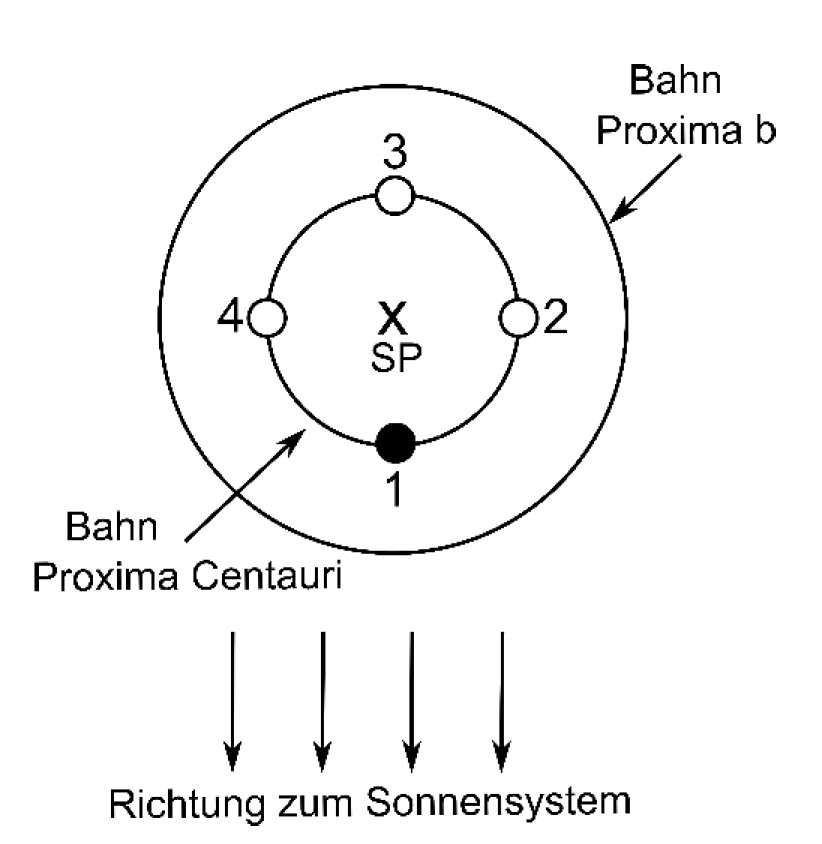
\includegraphics[width=0.3\textwidth]{Bilder/Proxima_schwerpunkt.jpg}{}
		\captionof{figure}{}\label{fig:Proxima-Schwerpunkt}
\end{aufgabe}

\begin{enumerate}
	\item Bei der Dopplerspektroskopie kann man die Geschwindigkeiten von Objekten im Weltall bestimmen. Spektroskopie bedeutet, dass man das von den Objekten ausgestrahlte Licht hinsichtlich seiner Wellenlängen, also seines Spektrums untersucht. Dabei vergleicht man das gemessene Spektrum mit Spektren die man auf der Erde genau vermessen kann. Man stellt fest, dass die Himmelsobjekte aus den gleichen Materialien aufgebaut sind, wie wir sie hier auf der Erde erzeugen können (bis auf wenige Ausnahmen, bei denen zu viel Energie nötig wäre). Vergleicht man das Spektrum eines ruhenden Körpers und eines Körpers, der sich vom Messpunkt wegbewegt, sind zwar die Abstände zwischen den Spektrallinien gleich, aber die Werte sind verschoben. Das liegt am Dopplereffekt. Dadurch kann umgekehrt auch durch Aufnahme des Spektrums die Geschwindigkeit eines Körpers gemessen werden, aber nur der vektorielle Anteil, mit dem sich der Körper wegbewegt und nicht zum Beispiel im Kreis bei gleichbleibendem Abstand. Solche Bewegungen, bei denen sich der Abstand ändert, nennt man Radialbewegungen. Insgesamt kann man also durch Messung der Spektren und Vergleich mit ruhenden Proben die Radialgeschwindigkeit von Himmelsobjekten bestimmen.
	
	Im Zweikörpersystem drehen sich beide beteiligten Körper um einen gemeinsamen Schwerpunkt. Kennt man die Bewegung dieses Schwerpunktes im Raum, so bewegen sich die beiden Körper mit dem Schwerpunkt mit, aber auch noch um den Schwerpunkt. Dadurch kommt es zu wellen- und schleifenförmigen Abweichungen von der Schwerpunktbewegung. So bewegen sich Erde und Mond um einen gemeinsamen Schwerpunkt, der innerhalb der Erde, aber nicht im Erdmittelpunkt liegt. Das gesamte System dreht sich aber noch um die Sonne und daher haben Mond noch Erde Abweichungen von perfekten Ellipsenbahnen im Orbit um die Sonne.

	Betrachtet man von der Erde aus einen Stern, so kann man seine Bewegung zum Beispiel mit Dopplerspektroskopie ermitteln. Hat dieser Stern keine Planeten, bewegt er sich ohne solche Störungen auf seiner Bahn relativ zur Erde. Hat er allerdings einen Planeten, mit dem er um einen gemeinsamen Schwerpunkt rotiert, kommen zu seiner Bahn periodische Veränderungen hinzu, die sich immer dann wiederholen, wenn der Planet einen Umlauf beendet hat. Diese Veränderungen kann man im Dopplerspektroskopiesignal messen und aufgrund der Geschwindigkeitsschwankungen auf einen Planeten schließen. 
	
	\item Die beiden Körper bewegen sich immer um einen Schwerpunkt, der zwischen ihnen liegt. Da der Schwerpunkt in der Abbildung genau im Zentrum der Kreisbahnen liegt, müssen die Körper sich jeweils genau gegenüber stehen, also um \ang{180} versetzt. \Cref{fig:Position} zeigt die dazugehörige Zeichnung.
	\begin{figure}
		\centering
		\begin{tikzpicture}
			\coordinate(orig) at (0,0);
			\coordinate (one) at (0,-1.5);
			\coordinate (two) at (1.5,0);
			\coordinate (three) at (0,1.5);
			\coordinate (four) at (-1.5,0);
			\draw (orig) pic{cross} node[right] {SP}  ;
			\draw
				(orig) circle (1.5)
				(orig) circle (3);
			\draw[text=white,draw=black,fill=black] (one) circle (0.5) node{1};
			\draw[text=black,draw=black,fill=white] (two) circle (0.5) node{2};
			\draw[text=black,draw=black,fill=white] (three) circle (0.5) node{3};
			\draw[text=black,draw=black,fill=white] (four) circle (0.5) node{4};
			\draw[text=white,draw=black,fill={rgb:red,150;green,150;blue,150}] (0,3) circle (0.5) node{1};
			\draw[->] (0,-3.5) -- ++ (0,-0.5) ;
			\draw[->] (-0.5,-3.5) -- ++ (0,-0.5) ;
			\draw[->] (0.5,-3.5) -- ++ (0,-0.5) ;
		\end{tikzpicture}
		\caption{Bahnen von Proxima b und Proxima Centauri um ihren gemeinsamen Schwerpunkt. Die äußere Bahn gehört zum Planeten Proxima b und die innere gehört zum Stern Proxima Centauri. Die Pfeile zeigen die Richtung an, in der unser Sonnensystem liegt, um den Bezug zu \cref{fig:radial} herzustellen.}
		\label{fig:Position}
	\end{figure}
	
	Um die Radialgeschwindigkeit als Funktion der Zeit zeichnen zu können, ist die Skizze der Orte zu verschiedenen Zeiten hilfreich. Da die Radialgeschwindigkeit die zeitliche Ableitung des Abstandes ist, bietet es sich an, zunächst die Abstände im Zeitverlauf aufzutragen.
	Das wurde im oberen Teil von \cref{fig:radial} gemacht. Hier wurde noch der Abstand $d_0$ des Schwerpunktes abgezogen, um die Schwingung um 0 zu zentrieren. Die Cosinus-Form des Abstandes kommt davon, dass man eine Kreisbewegung auf eine einzelne Richtung projiziert, nämlich die Beobachtungsrichtung. In Position 1 hat Proxima Centauri keine Abstandsveränderung, weil es dort am nächsten zur Erde steht und sich danach wieder wegbewegt. In Position 2 ist die Geschwindigkeit maximal mit positivem Vorzeichen, wenn man die Achsen so legt, dass positive Geschwindigkeiten zu größeren Abständen führen. In Position 3 findet man wieder einen Umkehrpunkt und in Position 4 maximale Geschwindigkeit in Richtung der Erde. Der untere Teil von \cref{fig:radial} zeigt den gesamten Zeitverlauf und deutet an, dass der Verlauf periodisch ist. Auch hier wurde wieder die Schwerpunktgeschwindigkeit $v_0$ abgezogen, um die Schwingung um 0 zu zentrieren. Zeichnerisch kann man die Punkte 1 bis 4 aus der Skizze ablesen und Cosinusförmig verbinden. Die Geschwindigkeit erhält man dann durch graphische Ableitung.



	\begin{figure}[t]
		\centering
		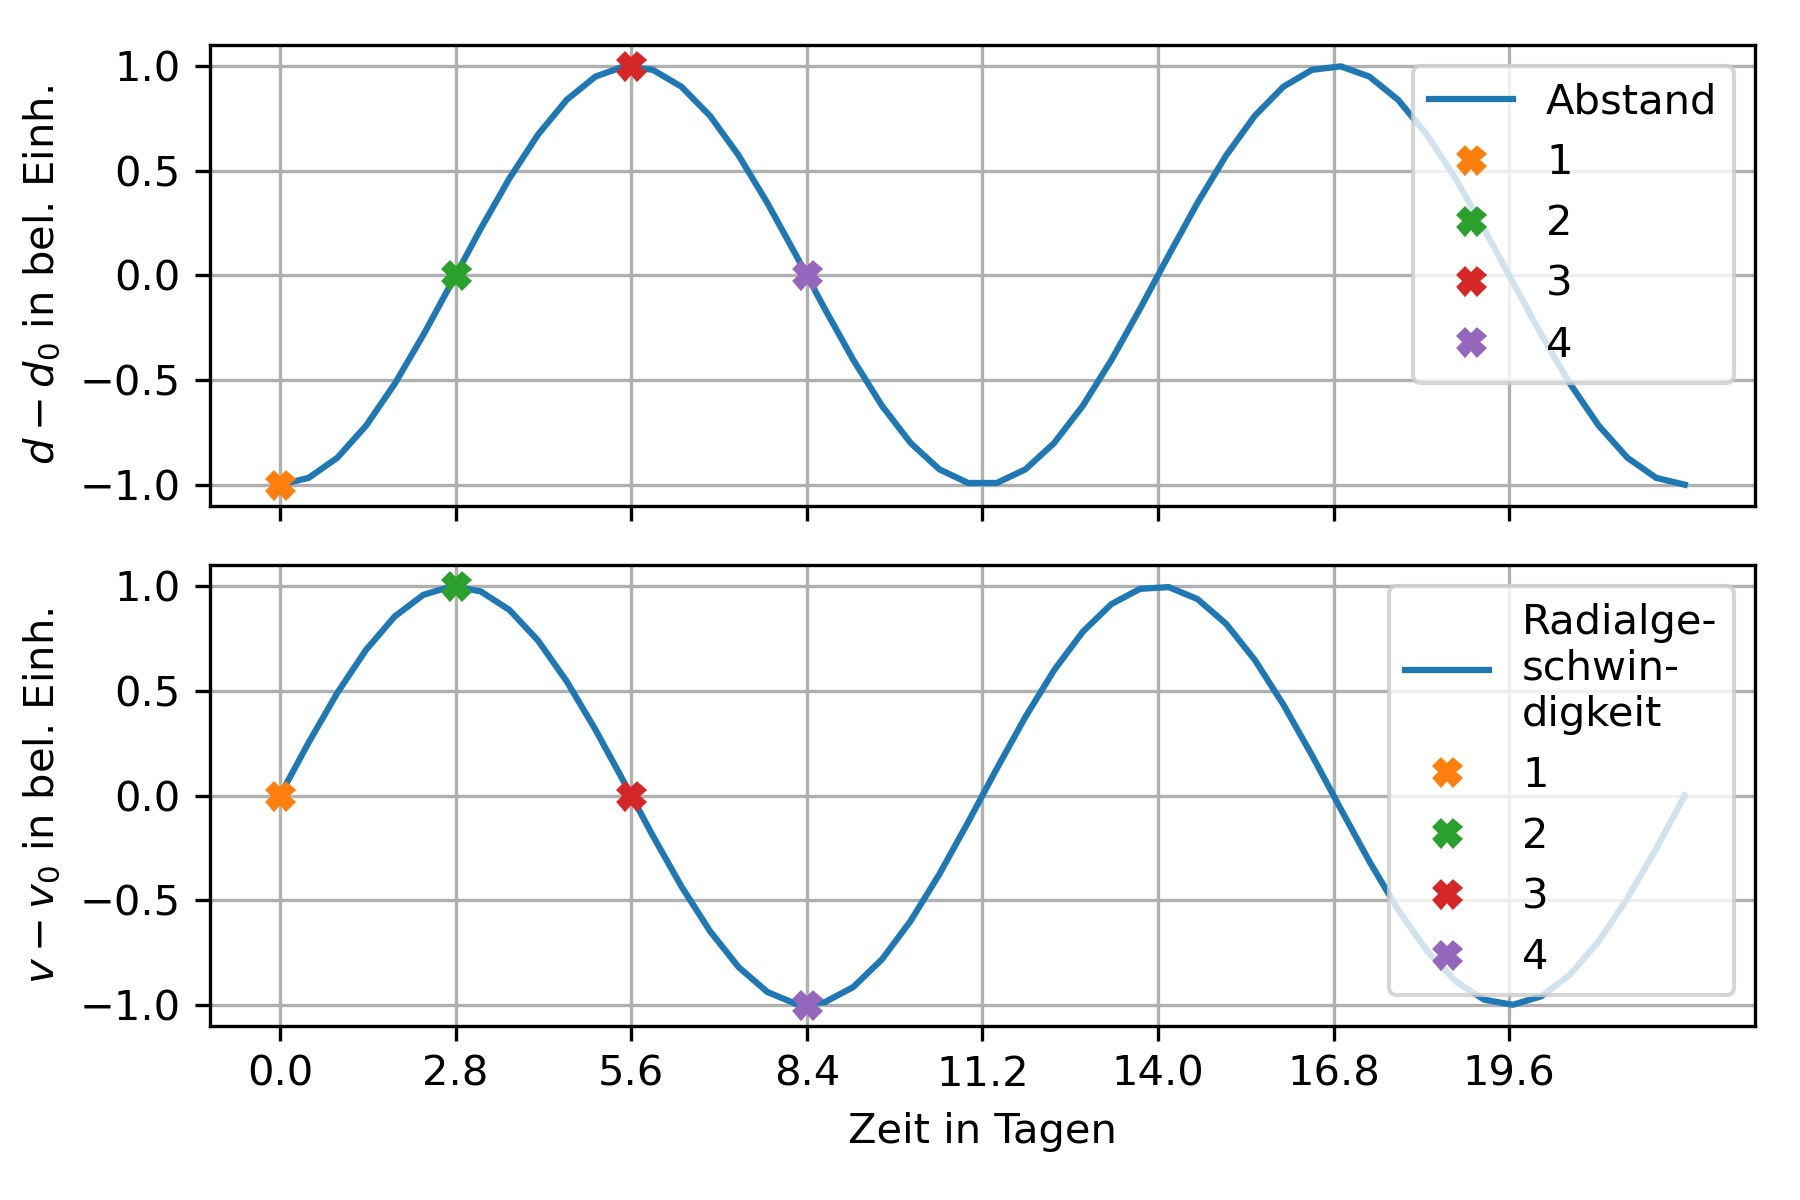
\includegraphics[width = 0.6\textwidth]{Bilder/radial.jpg}
		\caption{Radialbewegung von Proxima Centrauri im Zeitverlauf im System des gemeinsamen Schwerpunktes mit Proxima b. Im oberen Teil ist der Abstand $d$ zur Erde aufgetragen und der Abstand $d_0$ des Schwerpunktes abgezogen. Im unteren Teil ist die Radialgeschwindigkeit $v$ aus Sicht der Erde aufgetragen. Auch hier wurde die Radialgeschwindigkeit $v_0$ des Schwerpunktes abgezogen.  }
		\label{fig:radial}
	\end{figure}
	
	\item Die Bahn ist laut Angabe näherungsweise kreisförmig. Bei Kreisbewegungen muss immer eine Zentripetalkraft vorliegen, um den Körper in dieser Bewegung zu halten. Das liegt daran, dass eine Richtungsänderung der Geschwindigkeit immer durch eine Beschleunigung verursacht wird. Die Ursache für die Beschleunigung zur Mitte hin ist in diesem Fall die Gravitationskraft. Mit den Massen aus der Angabe und der Sonnen- und Erdmasse~\cite[S.47]{Cornelsen2013}, kann man die Kräfte berechnen. Für die Zentripetalkraft ist hier die Formel nützlich, in der die Kraft durch die Winkelgeschwindigkeit $\omega=\frac{2\pi}{T}$~\cite[S.11]{Cornelsen2013} ausgedrückt wird~\cite[S.12]{Cornelsen2013}, weil die Umlaufdauer $T$ bekannt ist. Es gilt:
	\begin{align*}
		F_G&=F_z\\
		G\frac{M_{\text{PC}}M_{\text{Pb}}}{r^2}&=M_{\text{Pb}}\omega^2r\\
		GM_\text{PC}&=\omega^2r^3\\
		r&=\sqrt[3]{\frac{GM_{\text{PC}}}{\omega^2}}\\
		&=\sqrt[3]{\frac{GM_{\text{PC}T^2}}{(2\pi)^2}}\\
		&=\sqrt[3]{\frac{\SI{6.67e-11}{\meter\cubed\per\kg\per\second\squared}\cdot \num{0.12}\cdot \SI{1.989e30}{\kg}\cdot \num{11.2}\cdot \SI{86400}{\second}}{4\pi^2}}\\
		&=\SI{7.2e9}{\meter}\\
		&\approx \SI{0.05}{\astronomicalunit}
	\end{align*}
	Der Planet, der unserer Sonne am nähsten ist, ist der Merkur mit einem Abstand von etwa \SI{0.387}{\astronomicalunit}~\cite[S.48]{Cornelsen2013}.
	Damit ist Proxima b deutlich näher an Proxima Centauri, als alle Planeten unseres Sonnensystems.

	\item Der Stern Proxima Centauri wird von Proxima b aus beobachtet. Dann erscheint der Stern am Himmel in einem Winkel $\varphi$, der durch den Radius $r_{\text{PC}}$ von Proxima Centauri und den Abstand $r$ zum Planeten gegeben ist. Die Trigonometrie liefert für den Winkel die Beziehung (siehe auch \cref{fig:Winkeldurchmesser}):
	\begin{align*}
		\tan(\varphi)=\frac{r_{\text{PC}}}{r}
	\end{align*}
	\begin{figure}
		\centering
		\begin{tikzpicture}
			\coordinate(proxb) at (-2,0.5);
		\coordinate (proxc) at (4,0.5);
		\draw (proxb) circle (0.25);
		\draw (proxc) circle(1.25);
		\draw[<->] (proxb) -- node[below]{$r$} (proxc) ;
		\draw[<->] (proxc) -- node[right]{$r_{\text{PC}}$} (4,1.75) coordinate(top);
		\draw[dashed] (proxb) -- (4,1.75);
		
		\draw pic [draw,->,"$\varphi$", angle radius = 3cm] {angle = proxc--proxb--top };
		\end{tikzpicture}
		\caption{Veranschaulichung der Argumentation zum Winkeldurchmesser. Beachte, dass die Abstände nicht maßstabsgetreu sind. Weil $r\gg r_{\text{PC}}$ ist es legitim von den Mittelpunkten der Himmelskörper auszugehen.}
		\label{fig:Winkeldurchmesser}
	\end{figure}
	Da der Abstand viel größer ist als der Radius handelt es sich um einen kleinen Winkel, deshalb gilt im Bogenmaß näherungsweise die Kleinwinkelnäherung $\varphi\approx \tan(\varphi)$~\cite[S.28]{Cornelsen2013}. Damit wird die obige Formel mit dem Erddurchmesser~\cite[S.47]{Cornelsen2013} und dem vorher berechneten Abstand zu
	\begin{align*}
		\varphi &= \frac{r_{\text{PC}}}{r}\\
		&=\frac{\num{0.15}\cdot\SI{6.957e8}{\meter}}{\SI{7.2e9}{\meter}}\\
		&=\SI{0.014}{\radian}
	\end{align*}
	Damit ist der Winkeldurchmesser durch $\alpha_\text{{PC}}=2\varphi=\SI{0.028}{\radian}$ gegeben. Das entspricht einem Winkel von
	\begin{align*}
		\alpha_{\text{PC}}&=\frac{\num{0.028}}{2\pi}\cdot \ang{360}=\ang{1.6}
	\end{align*}

	\begin{hinweis}
		Zur Erinnerung: Für Winkel gibt es in der Mathematik mehrere Maße. In der Physik kommt neben dem gut bekannten Gradmaß auch manchmal das Bogenmaß zum Einsatz. Beim Bogenmaß wird der Kreisbogen des Sektors des Einheitskreises gemessen. Manchmal gibt man dieses ohne Einheiten an, zur Verdeutlichung kann man es aber auch in seiner Einheit radian (\unit{\radian}) angeben. Die Kleinwinkelnäherung wie sie oben verwendet wurde, gilt nur für das Bogenmaß, denn $\tan(\ang{1.6})=\num{0.028}$. Hier sind Winkel und Tangens komplett verschiedene Zahlen, aber der Tangens stimmt gut mit dem Winkel im Bogenmaß überein.
	\end{hinweis}

	Zum Vergleich kann man die gleiche Rechnung für die Sonne machen. Mit dem Sonnenradius $r_\odot$~\cite[S.47]{Cornelsen2013} und dem Abstand von \SI{1}{\astronomicalunit} gilt:
	\begin{align*}
		\varphi_\odot&=\frac{r_\odot}{\SI{1}{\astronomicalunit}}=\frac{\SI{6.957e8}{\meter}}{\SI{1.496e11}{\meter}}=\SI{4.65e-3}{\radian}\\
		\alpha_\odot&=2\varphi_\odot=2\cdot\frac{\num{4.65e-3}}{2\pi}\cdot\ang{360}=\ang{0.53}
	\end{align*}
	Die Sonne erscheint daher an unserem Himmel kleiner als Proxima Centauri am Himmel von Proxima b.

	\item Die Bestrahlungsstärke ist gegeben durch die Leistung einer Lichtquelle, die auf eine bestimmte Fläche fällt. Betrachtet man einen Stern und seinen Planeten, so verteilt sich im Abstand des Planeten die gesamte Leistung des Sternes auf eine Kugeloberfläche. Die Kugel hat dabei als Radius genau den Abstand von Stern und Planet. Mit der Formel für die Kugeloberfläche gilt daher für die Bestrahlungsstärke $E$:
	\begin{align*}
		E&=\frac{L}{4\pi r^2}
	\end{align*}
	und diese Formel deckt sich mit der in~\cite[S.16]{Cornelsen2013}. Für Proxima Centauri und die Sonne ergibt sich dann auf ihren Planeten Proxima b und der Erde jeweils
	\begin{align*}
		E_{\text{Pb}}&=\frac{L_{\text{PC}}}{4\pi r_{\text{Pb}}^2}=\frac{\num{1.6e-3}\cdot\SI{3.846e26}{\watt}}{4\pi\cdot(\SI{7.2e9}{\meter})^2}=\SI{944.6}{\watt\per\meter\squared}\\
		E_\odot&=\frac{L_\odot}{4\pi r_{\text{Erde}}^2}=\frac{\SI{3.846e-26}{\watt}}{4\pi\cdot(\SI{1.496e11}{\meter})^2}=\SI{1367.5}{\watt\per\meter\squared}
	\end{align*}
	Dieser Wert stimmt genau mit dem Wert der Solarkonstante aus~\cite[S.47]{Cornelsen2013} überein. Bildet man das Verhältnis der beiden Werte, kommt man auf $\frac{E_{\text{Pb}}}{E_\odot}=\num{0.69}$, also kann man gut davon sprechen, dass die Bestrahlungsstärken auf den beiden Planeten in der gleichen Größenordnung liegen.

	\item Die Oberflächentemperatur hängt nicht nur von der Bestrahlungsstärke ab. Auf der Erde wird die Oberflächentemperatur maßgeblich von der Zusammensetzung der Erdatmosphäre beeinflusst. Sichtbares Licht kann die Atmosphäre gut durchdringen, wird auf der Erde absorbiert und als Wärme im Infraroten wieder abgestrahlt. Die infrarote Strahlung wird von der Atmosphäre jedoch nicht gut durchgelassen und es bleibt warm auf der Erde. Dieses Phänomen nennt man den Treibhauseffekt. Da Proxima Centauri im Infraroten strahlt und die Zusammensetzung der Atmosphäre von Proxima b hier nicht diskutiert wurde, ist unklar, ob es den Treibhauseffekt auch auf Proxima b gibt.
	
	Ein zweiter Einfluss auf die Oberflächentemperatur ist die Albedo. Dabei handelt es sich um die Oberflächenbeschaffenheit und wie sich diese auf die Reflexion von Strahlung auswirkt. Da hier die Oberfläche von Proxima b nicht betrachtet wurde, sind wir auch darüber in Unkenntnis.

	Ein dritter Einfluss (der hier eigentlich nicht verlangt ist), ist die Wärmeentstehung im Inneren der Planeten. Durch radioaktive Zerfalle und vulkanische Aktivität kann der Planet aus seinem Inneren heraus die Oberfläche erwärmen. Auch dieser Aspekt wurde hier nicht betrachtet.
	
\end{enumerate}